\subsection{Questionnaire and Results}\label{subsect:QuestionnaireResults}
To empirically validate our design hypothesis, the Google Forms survey was distributed to a varied sample of individuals involved in the fitness ecosystem. The questionnaire collected a total of 76 valid responses. By utilizing conditional logic branches within the form, we ensured that both gym members and professionals could provide specific, highly relevant insights based on their distinct operational contexts.

\subsubsection{Demographics}\label{subsubsect:Demographics}

\begin{figure}[H]
    \centering
    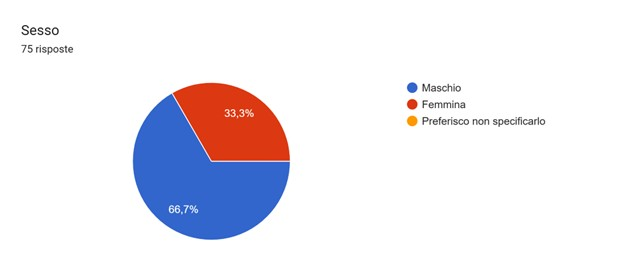
\includegraphics[width=0.8\textwidth]{3-UserResearch/img/Questionnaire/Demographics/Sesso.jpg}
    \caption{Gender distribution of the respondents.}
    \label{img:QuestionnaireGender}
\end{figure}

\begin{figure}[H]
    \centering
    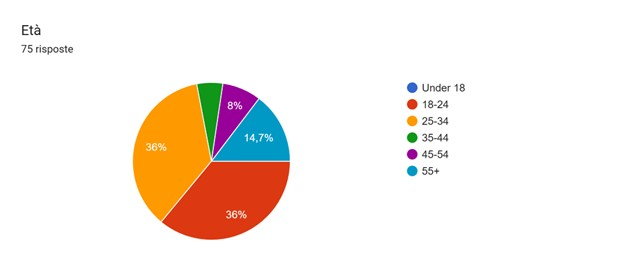
\includegraphics[width=0.8\textwidth]{3-UserResearch/img/Questionnaire/Demographics/Eta.jpg}
    \caption{Age distribution of the respondents.}
    \label{img:QuestionnaireAge}
\end{figure}

\begin{figure}[H]
    \centering
    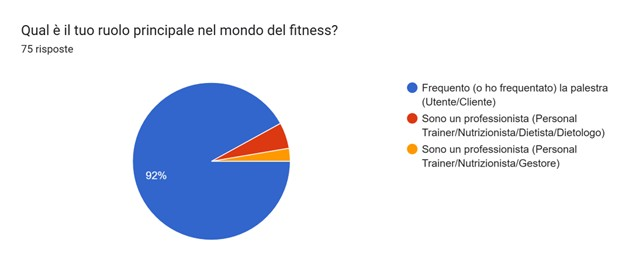
\includegraphics[width=0.8\textwidth]{3-UserResearch/img/Questionnaire/Demographics/Ruolo.jpg}
    \caption{Role distribution of the respondents.}
    \label{img:QuestionnaireRole}
\end{figure}

\textbf{Note: }The red and orange categories in the legend of Figure \ref{img:QuestionnaireRole} were split by Google Forms, but they actually represent the same group.

\vspace{0.3cm}
\textbf{Analysis of Demographics:} 
As shown in Figures \ref{img:QuestionnaireGender} and \ref{img:QuestionnaireAge}, the demographic profile of the respondents indicates a predominantly young adult audience, with the vast majority falling into the 18-24 and 25-34 age brackets. The sample of 76 respondents successfully captured insights from both sides of the market: exactly 92\% (70 individuals) identified as gym members (clients), while the remaining 8\% (6 individuals) are certified professionals (Personal Trainers, Nutritionists, and Dietitians). This specific distribution strongly mirrors the realistic proportions of a physical gym ecosystem, where a smaller, dedicated group of staff members manages a high volume of clients, ensuring that our feedback accurately reflects real-world market dynamics.


\subsubsection{Gym Members' Feedback}\label{subsubsect:GymMembers'Feedback}

\begin{figure}[H]
    \centering
    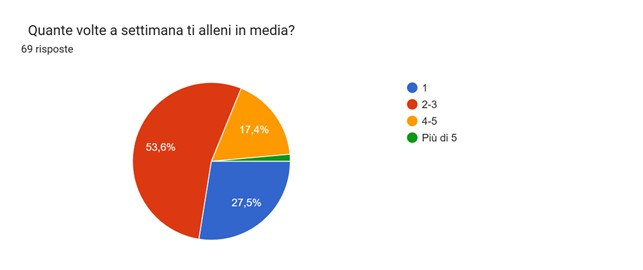
\includegraphics[width=0.8\textwidth]{3-UserResearch/img/Questionnaire/GymMembers/FrequenzaAllenamento.jpg}
    \caption{Frequency of training sessions.}
    \label{img:QuestionnaireFrequency}
\end{figure}

\begin{figure}[H]
    \centering
    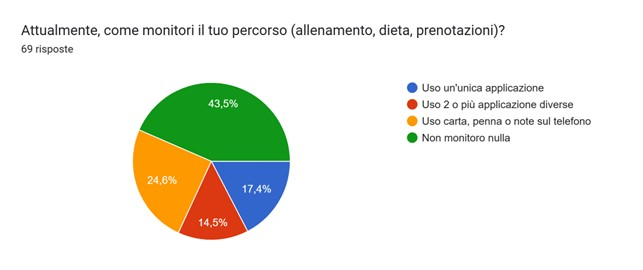
\includegraphics[width=0.8\textwidth]{3-UserResearch/img/Questionnaire/GymMembers/MonitoraggioAllenamento.jpg}
    \caption{Methods used by gym members to track their training sessions.}
    \label{img:QuestionnaireTracking}
\end{figure}

\begin{figure}[H]
    \centering
    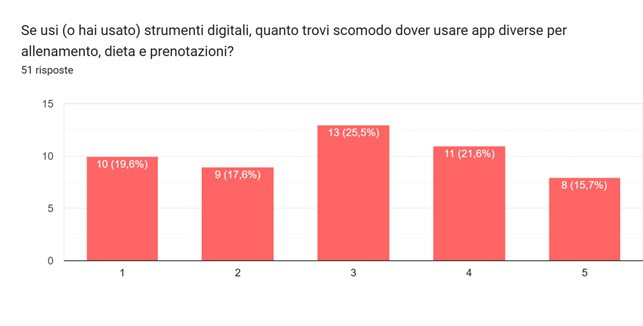
\includegraphics[width=0.8\textwidth]{3-UserResearch/img/Questionnaire/GymMembers/ScomoditaDiverseApp.jpg}
    \caption{Discomforts experienced by gym members when using different fitness apps.}
    \label{img:QuestionnaireDiscomfort}
\end{figure}

\begin{figure}[H]
    \centering
    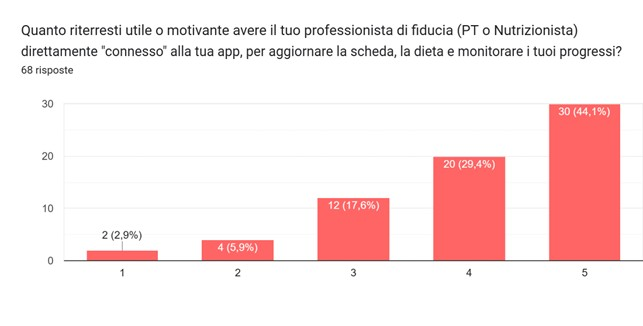
\includegraphics[width=0.8\textwidth]{3-UserResearch/img/Questionnaire/GymMembers/ConnnessioneProfessionista.jpg}
    \caption{Importance of connecting with a fitness professional.}
    \label{img:QuestionnaireConnection}
\end{figure}

\vspace{0.3cm}
\textbf{Analysis of Gym Members' Feedback:} 
The data reveals a highly active user base, with most participants training 2 to 5 times a week (Figure \ref{img:QuestionnaireFrequency}). Despite this dedication, Figure \ref{img:QuestionnaireTracking} highlights a critical inefficiency: a substantial portion of users still relies on analog methods (such as pen and paper or basic phone notes) or completely lacks a structured tracking system. Furthermore, many respondents suffer from the fragmentation of using multiple applications simultaneously. Consequently, Figure \ref{img:QuestionnaireDiscomfort} demonstrates the high frustration caused by this lack of integration. Most importantly, as depicted in Figure \ref{img:QuestionnaireConnection}, users expressed an overwhelming desire to have a direct, digital connection with their trusted professionals to receive updated diets and workout plans without constantly switching platforms.

\paragraph{Open Text Paragraph} Furthermore, the questionnaire included an open-ended question specifically directed at gym members, asking: \textit{"If you use one or more applications, please write their names in the field below"}. This specific inquiry proved to be extremely valuable for our overall market research. It allowed us to deepen and empirically validate the theoretical findings discussed during the Competitor Analysis phase (Chapter \ref{sect:CompetitorsAnalysis}). By collecting the exact names of the tools currently adopted by our real target audience, we were able to cross-reference our initial data, confirm our list of direct and indirect competitors, and ultimately prove the strong fragmentation that characterizes the current digital fitness landscape.


\subsubsection{Professionals' Feedback}\label{subsubsect:Professionals'Feedback}

\begin{figure}[H]
    \centering
    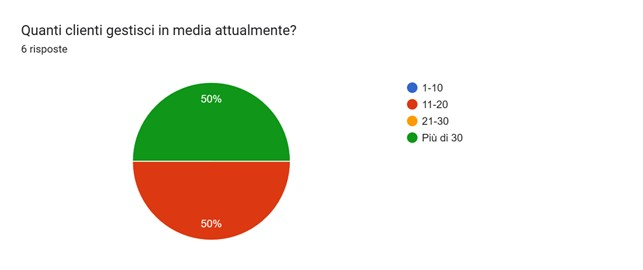
\includegraphics[width=0.8\textwidth]{3-UserResearch/img/Questionnaire/Professionists/NumeroClienti.jpg}
    \caption{Number of clients.}
    \label{img:QuestionnaireClients}
\end{figure}

\begin{figure}[H]
    \centering
    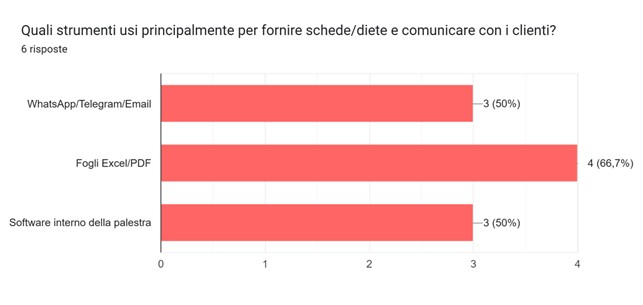
\includegraphics[width=0.8\textwidth]{3-UserResearch/img/Questionnaire/Professionists/StrumentiMonitoraggio.jpg}
    \caption{Tools used for monitoring clients.}
    \label{img:QuestionnaireMonitoring}
\end{figure}

\begin{figure}[H]
    \centering
    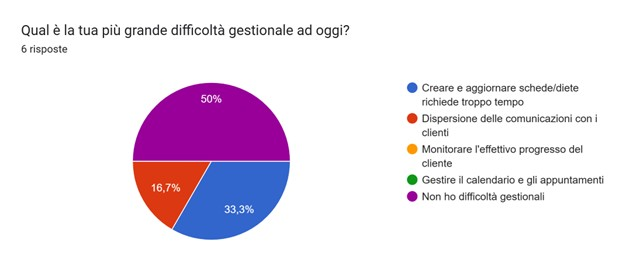
\includegraphics[width=0.8\textwidth]{3-UserResearch/img/Questionnaire/Professionists/DifficoltaGestionale.jpg}
    \caption{Challenges in client management.}
    \label{img:QuestionnaireChallenges}
\end{figure}

\vspace{0.3cm}
\textbf{Analysis of Professionals' Feedback:} 
The surveyed professionals manage varying client loads, ranging from a few individuals up to groups of over 50 clients (Figure \ref{img:QuestionnaireClients}). The core issue disrupting their workflow is clearly identified in Figure \ref{img:QuestionnaireMonitoring}: a heavy reliance on generic, non-specialized tools such as WhatsApp, Telegram, Emails, and Excel spreadsheets. Unsurprisingly, Figure \ref{img:QuestionnaireChallenges} confirms that their primary management challenges revolve around the dispersion of communications and the lack of constant, organized feedback from clients. Managing multiple user routines through chaotic messaging applications creates an unsustainable administrative burden, strongly proving the necessity for a centralized professional dashboard.


\subsubsection{User Expectations and Proposed Solutions}\label{subsubsect:CommonFeedback}

\begin{figure}[H]
    \centering
    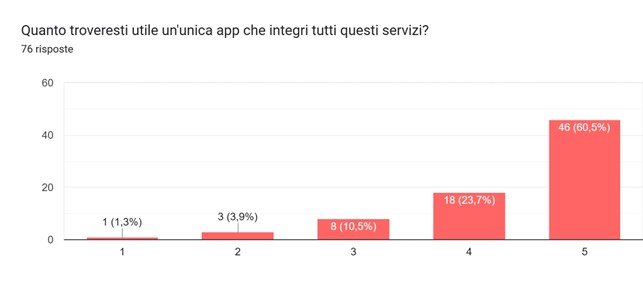
\includegraphics[width=0.8\textwidth]{3-UserResearch/img/Questionnaire/Common/UtilitaIntegrazione.jpg}
    \caption{Perceived usefulness of integrating a fitness app with a professional's monitoring system.}
    \label{img:QuestionnaireIntegration}
\end{figure}

\begin{figure}[H]
    \centering
    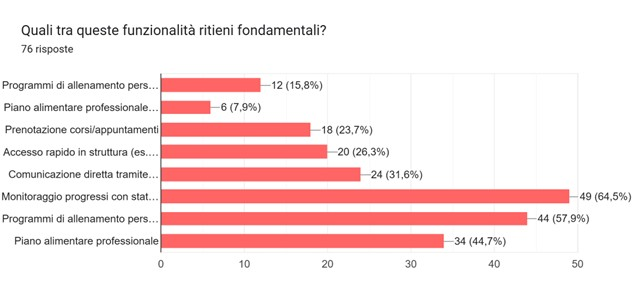
\includegraphics[width=0.8\textwidth]{3-UserResearch/img/Questionnaire/Common/FunzionalitaFondamentali.jpg}
    \caption{Essential features for a fitness app integrated with a professional's monitoring system.}
    \label{img:QuestionnaireEssentialFeatures}
\end{figure}

\vspace{0.3cm}
\textbf{Analysis of Expectations:} 
When asked about the potential utility of an all-in-one application that aggregates all these scattered services, the response was incredibly positive: Figure \ref{img:QuestionnaireIntegration} shows an overwhelming approval rating from both clients and professionals. Regarding the core functionalities (Figure \ref{img:QuestionnaireEssentialFeatures}), respondents pinpointed personalized workout tracking, professional diet management, and rapid digital facility access as absolute must-haves. These results definitively validate our initial feature assumptions and provide a clear, user-approved roadmap for TrainHub's core architecture.

\subsubsection{Qualitative Insights and Methodological Refinement}\label{subsubsect:QualitativeInsights}

\paragraph{Uncovering Unmet Needs and Feature Elicitation}
To maximize the value of our user research, the survey included an open-ended question designed to uncover specific pain points: \textit{"If you could improve or solve an impractical aspect related to the digital experience in the gym, what would it be?"}. Rather than directly asking participants what features they wanted, this problem-oriented approach allowed us to indirectly elicit new and unanticipated functional requirements. By focusing on the users' real frustrations and daily friction points, we gathered organic insights into unmet needs. This qualitative data significantly enriched the conceptualization of TrainHub, helping us identify and prioritize secondary features that could further elevate the platform's value proposition.

\paragraph{Methodological Feedback and Iterative Improvement}
Finally, acknowledging our ongoing learning process as university students, we added a concluding section dedicated entirely to methodological feedback: \textit{"Being a university project, we are still learning how to conduct user research. If you found any question unclear or hard to interpret, please let us know. Every feedback is gold to us!"}. This meta-research inquiry proved to be incredibly valuable in practice. The constructive criticism received from the earliest respondents highlighted minor ambiguities in our initial phrasing. Consequently, we adopted an agile and iterative approach, actively fine-tuning and adjusting the questionnaire during the data collection phase. This continuous refinement ensured maximum clarity for subsequent participants, thereby increasing the overall reliability and accuracy of our final dataset.